% cuBLAS 库
% CUDA|GPU 编程|BLAS|线性代数

本词条将大致介绍如何使用 CUBLAS 库,同时演示一个使用 CUBLAS 库进行矩阵乘法的例子.
\subsection{CUDA 的安装}
请参阅 nvidia 官方文档或你的发行版文档.

如:ArchLinux 通过
\begin{lstlisting}[language=cpp]
pacman -S cuda
\end{lstlisting}
一条命令安装.

\begin{figure}[ht]
\centering
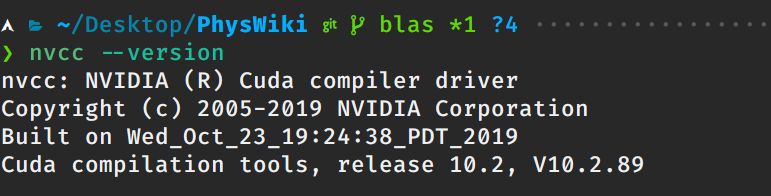
\includegraphics[width=12cm]{./figures/cublas_3.png}
\caption{测试 nvcc} \label{cublas_fig3}
\end{figure}

\subsection{CUBLAS 内容}%
%\label{sec:cublas_nei_rong_}

CUBLAS 是 CUDA 专门用来解决线性代数运算的库,它分为三个级别(见 blas)

同时该库还包含状态结构和一些功能函数.

\subsection{CUBLAS 用法}%
%\label{sec:cublas_yong_fa_}

大体分成以下几个步骤:

\begin{enumerate}
  \item 定义 CUBLAS 库对象 
  \item  在显存中为待运算的数据以及需要存放结果的变量开辟显存空间(\verb|cudaMalloc| 函数实现)
  \item  将待运算的数据传输进显存(\verb|cudaMemcpy|,\verb|cublasSetVector| 等函数实现)
  \item 调用 CUBLAS 库函数(根据 CUBLAS 手册调用需要的函数)
  \item 从显存中获取结果变量(\verb|cudaMemcpy|,\verb|cublasGetVector| 等函数实现)
  \item  释放申请的显存空间以及 CUBLAS 库对象(cudaFree 及 cublasDestroy 函数实现)
\end{enumerate}

\subsection{代码示例}%
%\label{sub:dai_ma_shi_li_}

使用 CUBLAS 库进行矩阵乘法运算

如果你的文本编辑器是 vim, 推荐使用 ale, ycm, Asynctask 来做 cuda 的语法检查,语义补全,项目管理工具.
\begin{lstlisting}[language=cpp, caption=cublas\_demo.cu]
// CUDA runtime 库 + CUBLAS 库 
#include "cuda_runtime.h"
#include "cublas_v2.h"

#include <time.h>
#include <iostream>

using namespace std;

// 定义测试矩阵的维度
int const M = 5;
int const N = 10;

int main(void) 
{   
    // 定义状态变量
    cublasStatus_t status;

    // 在 内存 中为将要计算的矩阵开辟空间
    float *h_A = (float*)malloc (N*M*sizeof(float));
    float *h_B = (float*)malloc (N*M*sizeof(float));
    
    // 在 内存 中为将要存放运算结果的矩阵开辟空间
    float *h_C = (float*)malloc (M*M*sizeof(float));

    // 为待运算矩阵的元素赋予 0-10 范围内的随机数
    for (int i=0; i<N*M; i++) {
        h_A[i] = (float)(rand()%10+1);
        h_B[i] = (float)(rand()%10+1);
    
    }
    
    // 打印待测试的矩阵
    cout << "矩阵 A :" << endl;
    for (int i=0; i<N*M; i++){
        cout << h_A[i] << " ";
        if ((i+1)%N == 0) cout << endl;
    }
    cout << endl;
    cout << "矩阵 B :" << endl;
    for (int i=0; i<N*M; i++){
        cout << h_B[i] << " ";
        if ((i+1)%M == 0) cout << endl;
    }
    cout << endl;
    
    /*
    ** GPU 计算矩阵相乘
    */

    // 创建并初始化 CUBLAS 库对象
    cublasHandle_t handle;
    status = cublasCreate(&handle);
    
    if (status != CUBLAS_STATUS_SUCCESS)
    {
        if (status == CUBLAS_STATUS_NOT_INITIALIZED) {
            cout << "CUBLAS 对象实例化出错" << endl;
        }
        getchar ();
        return EXIT_FAILURE;
    }

    float *d_A, *d_B, *d_C;
    // 在 显存 中为将要计算的矩阵开辟空间
    cudaMalloc (
        (void**)&d_A,    // 指向开辟的空间的指针
        N*M * sizeof(float)    // 需要开辟空间的字节数
    );
    cudaMalloc (
        (void**)&d_B,    
        N*M * sizeof(float)    
    );

    // 在 显存 中为将要存放运算结果的矩阵开辟空间
    cudaMalloc (
        (void**)&d_C,
        M*M * sizeof(float)    
    );

    // 将矩阵数据传递进 显存 中已经开辟好了的空间
    cublasSetVector (
        N*M,    // 要存入显存的元素个数
        sizeof(float),    // 每个元素大小
        h_A,    // 主机端起始地址
        1,    // 连续元素之间的存储间隔
        d_A,    // GPU 端起始地址
        1    // 连续元素之间的存储间隔
    );
    cublasSetVector (N*M, sizeof(float), h_B, 1, d_B, 1);

    // 同步函数
    cudaThreadSynchronize();

    // 传递进矩阵相乘函数中的参数,具体含义请参考函数手册.
    float a=1; float b=0;
    // 矩阵相乘.该函数必然将数组解析成列优先数组
    cublasSgemm (
        handle,    // blas 库对象 
        CUBLAS_OP_T,    // 矩阵 A 属性参数
        CUBLAS_OP_T,    // 矩阵 B 属性参数
        M,    // A, C 的行数 
        M,    // B, C 的列数
        N,    // A 的列数和 B 的行数
        &a,    // 运算式的 \alpha 值
        d_A,    // A 在显存中的地址
        N,    // lda
        d_B,    // B 在显存中的地址
        M,    // ldb
        &b,    // 运算式的 \beta 值
        d_C,    // C 在显存中的地址(结果矩阵)
        M    // ldc
    );
    
    // 同步函数
    cudaThreadSynchronize();

    // 从 显存 中取出运算结果至 内存中去
    cublasGetVector (
        M*M,    //  要取出元素的个数
        sizeof(float),    // 每个元素大小
        d_C,    // GPU 端起始地址
        1,    // 连续元素之间的存储间隔
        h_C,    // 主机端起始地址
        1    // 连续元素之间的存储间隔
    );
    
    // 打印运算结果
    cout << "计算结果的转置 ( (A*B)的转置 ):" << endl;

    for (int i=0;i<M*M; i++){
            cout << h_C[i] << " ";
            if ((i+1)%M == 0) cout << endl;
    }
    
    // 清理掉使用过的内存
    free (h_A); free (h_B); free (h_C); cudaFree (d_A);
    cudaFree (d_B); cudaFree (d_C);

    // 释放 CUBLAS 库对象
    cublasDestroy (handle);
    return 0;
}
\end{lstlisting}

\begin{figure}[h]
\centering
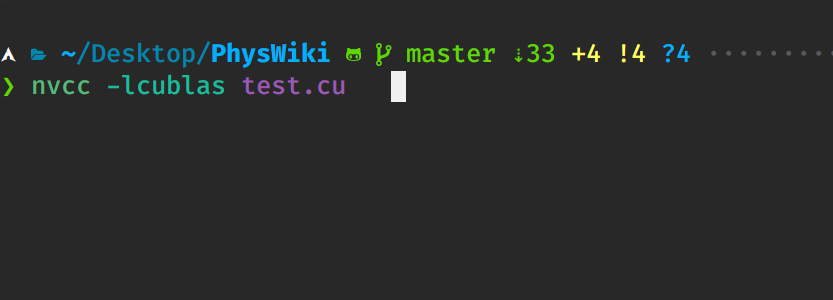
\includegraphics[width=11cm]{./figures/cublas_1.png}
\caption{编译} \label{cublas_fig1}
\end{figure}

\begin{figure}[h]
\centering
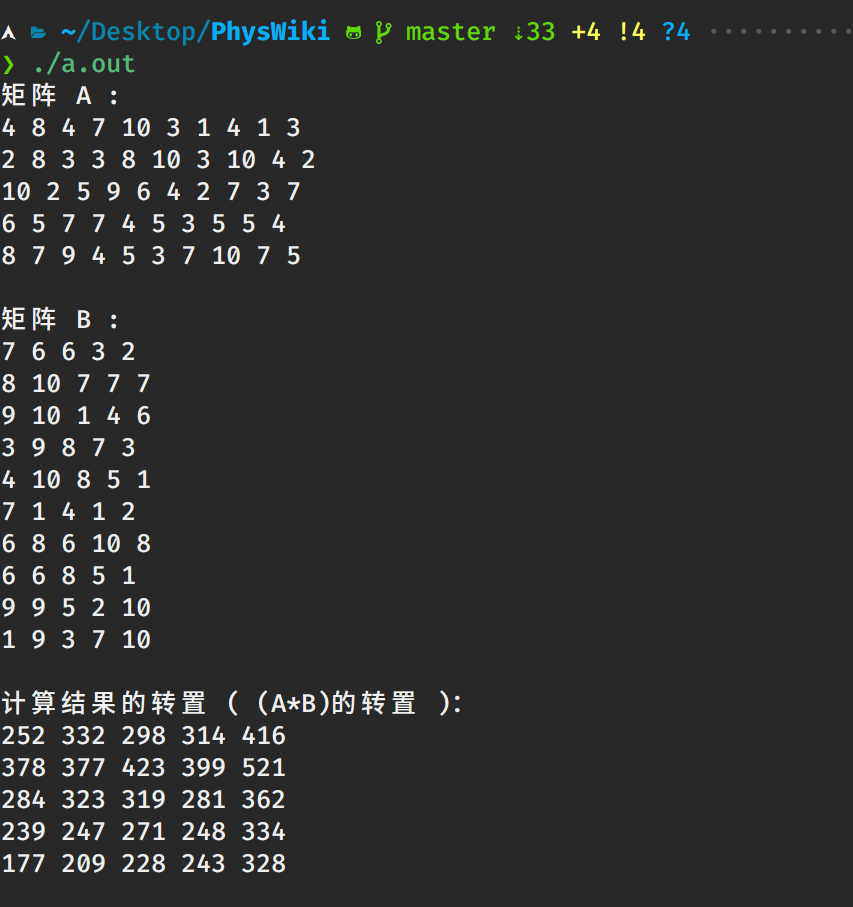
\includegraphics[width=11cm]{./figures/cublas_2.png}
\caption{运行} \label{cublas_fig2}
\end{figure}

\subsection{cublas 文档}%
%\label{sub:cublas_wen_dang_}

cuda 的文档十分易懂,内有丰富的例子.

我将 cuda 安装在 \verb|/opt| 下, 那么 cublas 库的文档就在 \verb|/opt/cuda/doc/cublas| 下.

